\clearpage
\chapter{Introduction}
\label{sec:intro}

Performing experiments is a key component of human development and has been the foundation of knowledge gain during the evolution of mankind. However, the exchange of such experimental results requires the long term documentation of the  experimental procedure. This is only possible with the means of writing down the experimental purpose, execution and result since the invention of scripture. Nowadays, tideous manual scripture has largely been replaced by digital information, making information easier transportable, searchable and duplicatable. Therefore all scientific research nowadays relies mainly on digital information acquisition and storage. Although data can be easily stored and transferred with modern technologies, interpretation of research data is not straight forward as datasets are highly diverse between scientific areas. Depending on the area of research, the diversity within a field highly depends on the field, e.g. in fields which require large experimental setups (particle physics / high field FMRI) data formats and structures  there are only a few data formats defined by the community / company producing the corresponding setup. In other fields the diversity of data is bigger since the scientific methods and aims require a diversity of approaches. Unification would require organizational large-scale efforts arcoss the community and implies additional overhead on the level of each experiment. In this thesis I discuss approaches for data and metadata management for efficient and robust handling of research data from data aquisition to analyis.

The diversity in data modalities and file formats promotes also a heterogeneity in data analysis steps and tools used for extraction of scientific findings.

\todo{TODO: go on here with describing need to standardize analyses and the requirement of complete / consistent metadata}
\todo{Introduce: Reproducible vs replicable vs ...}

\todo{Introduce odML, nix, ...}


\section{Data and metadata models}
Standardization of data and metadata is a fundamental requirement for the usability of data and metadata. This work is based on two common, generic models for capturing metadata and data. Both software projects are developed and maintained by the German Neuroinformatics Node (G-Node) an organization aiming to improve the infrastructure for data access, data storage and data analysis. 

\subsection{Hierarchical metadata in the \software{odML} model}
\label{sec:subodML}

odML\footnote{\url{https://github.com/G-Node/python-odml}, RRID:SCR\_001376} is a versatile hierarchical format for metadata \citep{Grewe_2011}. While it was originally designed for electrophysiological metadata, its generic structure makes it also applicable to other scientific contexts.

The basic concept is to use a tree-like structure of \code{Section}s to store metadata as \code{Properties} (extended key-value pairs) in a common \code{Document} (\cref{fig:intro_odML_structure}). The \code{Document} captures the general metadata regarding the metadata collection: the author of the collection, the date of generation, a custom version specifier and a custom reference repository. The hierarchical structure of the collection is formed by \code{Section}s which can be concatenated to build the branches of a tree structure (\cref{fig:intro_odML_model}). Here, each \code{Section} carries information about the subset of metadata it contains in form of a \code{Section} name providing a brief categorization, a definition extending on the category typically in form a complete senctence and a type for grouping across \code{Section}s. Additionally a \code{Section} can also point to an external repository or reference (e.g. a data base) or link or include parts of other \software{odML} structures. \code{Properties} provide with their name attribute the key corresponding to the stored metadata values. Each \code{Property} contains a list of value entries and gathers the corresponding metadata as its \code{Property} attributes. E.g. the data type (dtype), physical unit, uncertainty and value origin are shared between all metadata values of a \code{Property}. Same as the \code{Section} also the \code{Property} can carry a human-readable description of the values contained and can also reference to an external location. The value of a \code{Property} can also depend on another \code{Property} (dependency attribute) or another  value (dependency\_value attribute). All \software{odML} objects carry a universally unique identifier (UUID, auto-generated identifier with extremely low collision probability) for unique identification of odML entities even across unrelated files to ensure comprehensive provenance tracking. This permits the referencing and inclusion across projects.

For example, using this paradigm, the metadata of an experiment can be grouped on a first level of \code{Section}s in to hardware related or non-hardware related. For each of these groups the separation by either different hardware components or experiment aspects makes sense. On the next level a diversification by more detailed aspects like the subcomponents of the hardware or manual versus static parameters can be implemented. Finally, the manual parameters of a specific device used in an experiment can be represented as \code{Properties} collected in a specific \code{Section}. Whereas another branch of the \software{odML} structure contains \code{Properties} describing the subject performing the experiment, e.g. in \code{Properties} containing the age, gender, handedness, etc.

\todo{The usage of \software{odML} in different environments with varying requirements has led to diversification, the identification of unused features, and the need for improvement of the original data model.}

\begin{figure}
    \centering
    \includestandalone[mode=image|tex, width=0.7\textwidth, obeyclassoptions=true]{./figures/introduction/odML_structure}
    \caption[\software{odML} structure and objects]{\software{odML} structure and objects. \software{odML} provides three objects for metadata organization: The \software{odML} \code{Document} forms the basis of a hierarchy for metadata storage. It can link to a number of \software{odML} \code{Section}s. \code{Section}s are used to build a hierarchical structure and to provide context and relation between metadata. Each \code{Section} can link to multiple \code{Properties}. These contain the actual metadata values accompanied by essential information providing the context for interpretation of the values.}
    \label{fig:intro_odML_structure}
\end{figure}

\begin{figure}
    \centering
    \includesvg[width=0.7\textwidth]{./figures/introduction/odML_DataModel_escus}
    \caption[\software{odML} model]{\software{odML} model. \code{Document}s and \code{Section}s can link to multiple of their child attributes, whereas each object has exactly one parent objects, generating a branching, hierarchical structure. Each object has an identifier \software{odML} for unique identification across files. The \code{Document} additionally contains general metadata collection attributes to store the author, the version, the generation date and the corresponding repository reference. The \code{Section} describes provides common information about the contained child \code{Section}s and \code{Properties}. The \code{Property} name acts as key associated to the actual metadata value stored. Additionally the \code{Property} provides supplementary essential information for the interpretation of the metadata value.}
    \label{fig:intro_odML_model}
\end{figure}

\paragraph{Additional features}
The \software{odML} core library already provides an in-built mechanism to search and retrieve \code{Section}s, \code{Propertie}s or values within a \code{Document}. The need to consistently search for metadata entities across Documents from different sources led to the development of an export feature of \software{odML} metadata to the Resource Description Framework (RDF) format\footnote{\url{http://www.w3.org/TR/rdf-primer}}, a general and widely used storage format of graph databases. Multiple \software{odML} files exported to RDF can be loaded into any graph database supporting RDF and will be combined into a single graph. Moreover, while XML is still the default storage format, \software{odML} now additionally supports storing the metadata in the text based file formats JSON\footnote{\url{https://json.org}} and YAML\footnote{\url{https://yaml.org}}. JSON has become a de-facto data exchange standard between web based and standalone computer applications. The support of JSON makes \software{odML} metadata more easily consumable in machine-only workflows through modern applications. Since both XML and JSON primarily aim at machine-readability, their structure is not easily readable by humans. To ease reading of raw \software{odML} files by actual persons the YAML file format support was added.

For easy visualization and manipulation of specific \software{odML} files, the graphical user interface of \software{odMLtables} (\cref{sec:metadata}) was integrated into the native \software{odML} GUI (odml-ui\footnote{\url{https://github.com/G-Node/odml-ui}}). Thus, the \software{odML} GUI now grants direct access to the main \software{odMLtables} features, making both software tools even easier to use back to back for both browsing and editing of metadata.


\subsection{Generic data organization via the \software{Nix} model}
The \software{Nix} model combines data and metadata in a common framework. For this six generic data objects are defined and combined with an \software{odML} based metadata structure. The \software{Nix} model is provided with a \software{C++} reference implementation\footnote{nixio \software{C++}, \url{https://nixio.readthedocs.io},  RRID:SCR\_016196} and bindings for \software{Java}, \software{Matlab}. An independent implementation in \software{Python} is provided\footnote{nixio / nixpy, Python, \url{https://pypi.org/project/nixio/}} with version $1.5.0b3$ being considered here.

The \software{Nix} model consists of two different types of object for the description of data and metadata. In total, there are six data and two metadata objects  described in the following (\ref{fig:intro_nix_model}).
Data values are caputured using \code{DataArray}s capable of holding any type of data that can be described using a single or multidimensional array. In addition to the values the \code{DataArray} also describes the physical properties of the stored values, e.g. the type of data, the physical unit of the values and a human readable label. Additionally the data array is connected to \code{Dimension} objects, providing details about each of the additional dimensions of the \code{DataArray} including also a label, the physical unit, a sampling interval and offset. With these two objects \software{Nix} captures all required data for a meaningful visualization of the stored data values (e.g. see \cref{fig:intro_nix_examples}). In addition, it offers objects for tagging subsets of the values stored in a \code{DataArray} and for describing the origin of the recording data. The first one is implemented as a \code{Tag} object, referencing a subset of the values in a \code{DataArray} and can be used to provide more information for a subset of values, e.g. the presentation of a stimulus or the labelling of a cell part. The second object is a \code{Source} object, which is used to track the origin of data. The remaining data object \code{Group} is used for logical grouping of other \software{Nix} data objects. All data objects are coordinated via \code{Block}, which again is together with the metadata objects grouped in a \software{Nix} \code{File} object, representing a complete dataset.
The metadata objects used in the \software{Nix} framework are taken from the \software{odML} framework. All data objects within \software{Nix}, except for the \code{Dimension} object, can link to a single \code{Section} in the metadata collection of the \software{Nix} \code{File}, which contains additional information about the data object. Depending on the declared types of the linked data and metadata object, this relation is interpreted mono- or bidirectional, i.e. the metadata \code{Section} enriches the data object or the metadata object is additionally also defined via the data object.

The \software{Nix} repository is accompanied with an extensive wiki\footnote{\software{Nix} wiki, \url{https://github.com/G-Node/nix/wiki}} and documentation\footnote{\software{Nix} documentation, \url{https://nixio.readthedocs.io}} including tutorials and demos, providing detailed user-level documentation.

The \software{Nix} model is natively integrated in the the electrophysiology recording system \software{RELACS}, the \software{EEGbase}\footnote{EEGbase, \url{http://eegdatabase.kiv.zcu.cz}, RRID:nif-0000-08190} a system for storage, management, sharing and retrieval of EEG data as well as \software{Neo}, a Python tool for standardized representation of electrophysiology data (\ref{sec:neo}).


\begin{figure}
 \centering
 \begin{minipage}[t]{0.8\textwidth}
 \textbf{A}\newline\\
 \hfill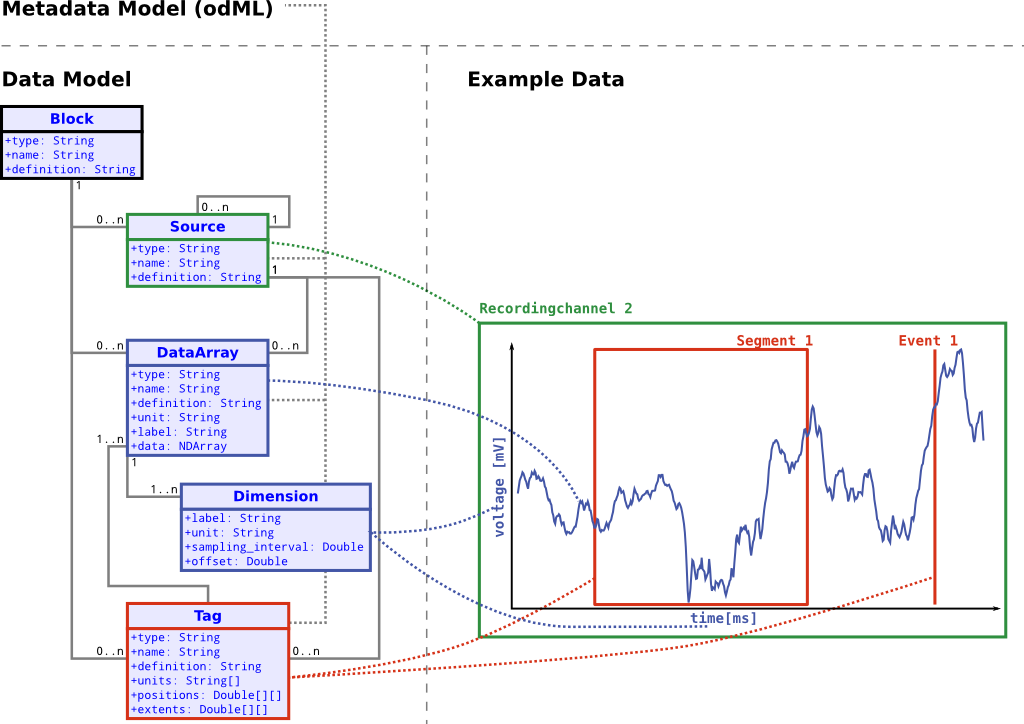
\includegraphics[width=0.9\textwidth]{./figures/introduction/pandora_example_signal}
 \end{minipage}\\
 \vspace{1cm}
 \begin{minipage}[t]{0.8\textwidth}
 \textbf{B}\newline\\
 \hfill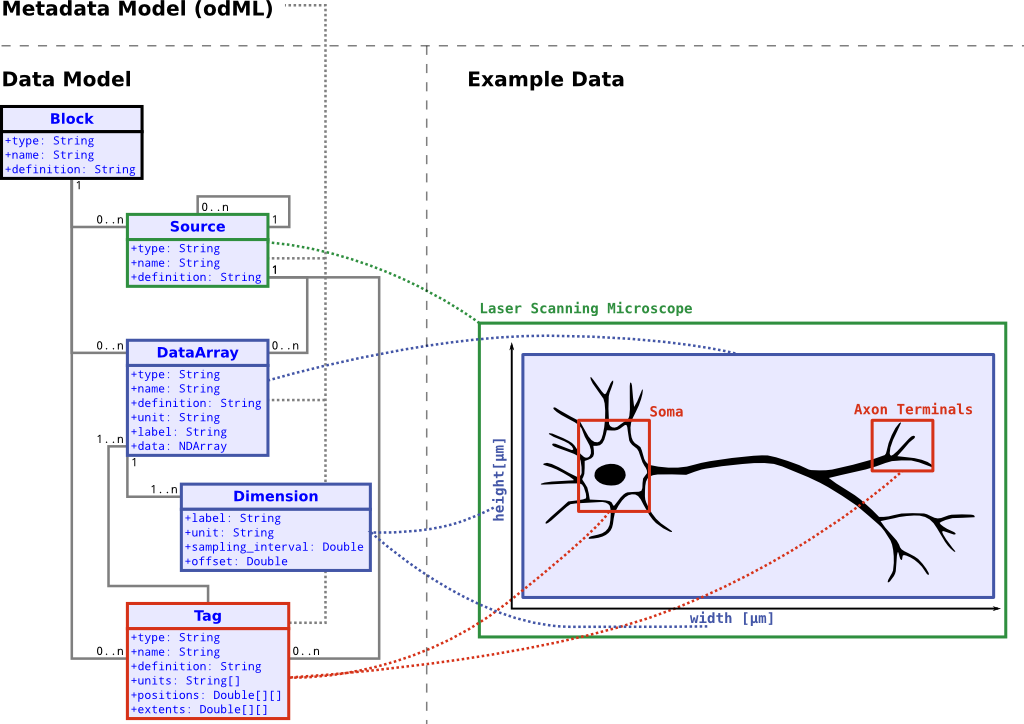
\includegraphics[width=0.9\textwidth]{./figures/introduction/pandora_example_image}
 \end{minipage}
 \caption[Nix model application examples]{Nix model application examples. The model can capture different varieties of data, e.g. electrophysiological recording traces (A) and imaging data (B). Both signals types can be mapped to the same types of objects of the \software{Nix} model. Figure from \software{Nix} documentation\footnote{\url{https://github.com/G-Node/nix/wiki/The-Model}}}
 \label{fig:intro_nix_examples}
\end{figure}

\begin{figure}
 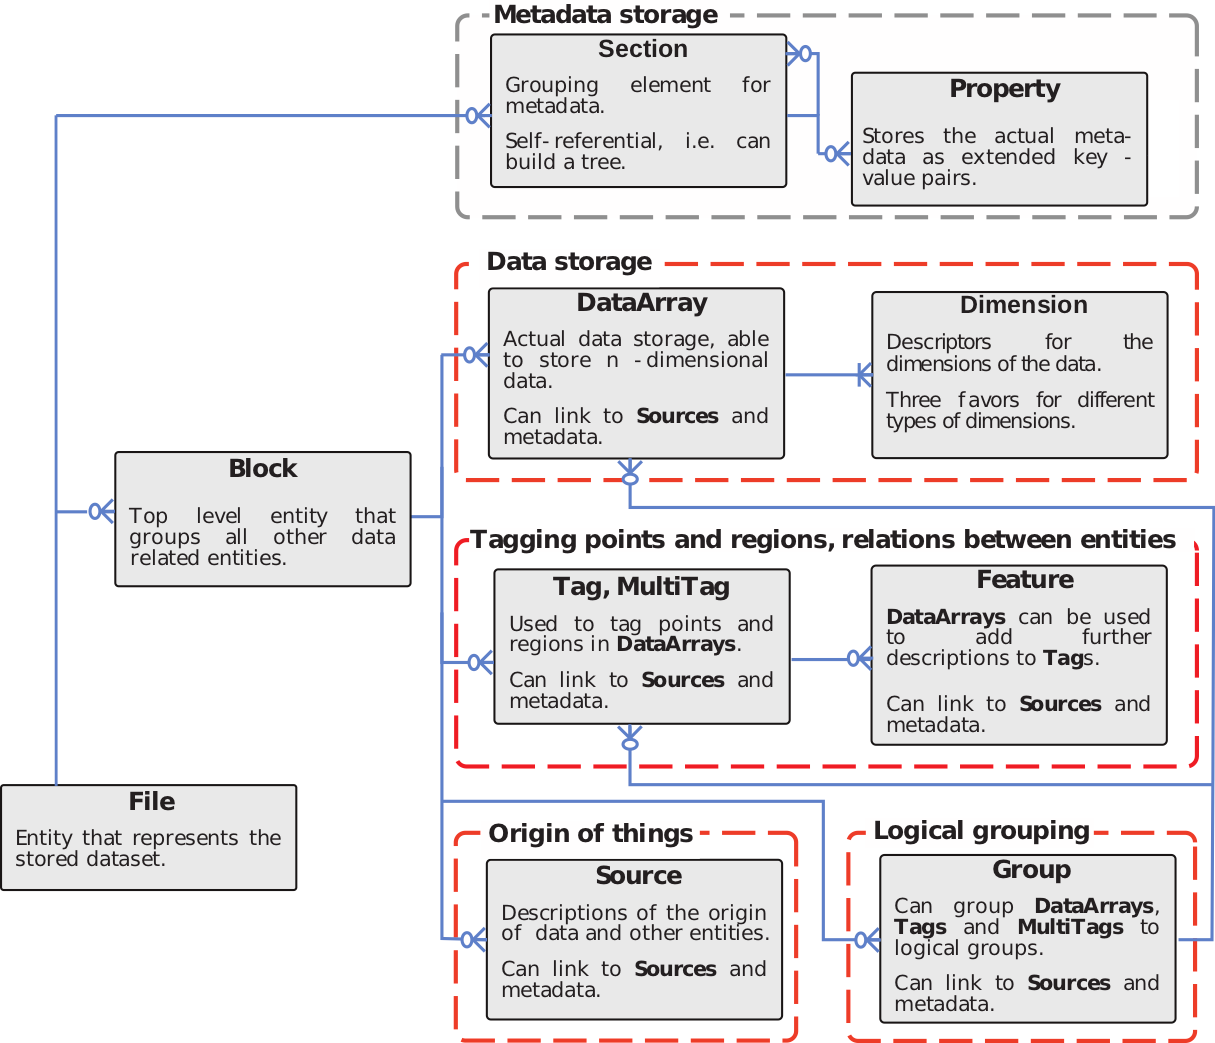
\includegraphics[width=0.9\textwidth]{./figures/introduction/data_model_brief_adapted}
 \caption[Nix model objects]{Nix model objects. The model consist of objects for storing data and metadata and relations between these. Metadata is captured in a \software{odML} based structure. Figure adapted from \software{Nix} documentation\footnote{\url{https://nixio.readthedocs.io/en/latest/data_model.html}}}
 \label{fig:intro_nix_model}
\end{figure}

\section{Thesis overview}
In \cref{sec:data} we describe two published datasets of a complex, collaborative electrophysiological experiment including an extensive metadata collection. We describe the process of data and metadata preparation required for the data publication and discuss the workflow used in this publication to identify strengths and shortcomings of the presented approach. In \cref{sec:metadata} we present odMLtables, a tool for facilitation of metadata collection compatible with the previously presented workflow. We demonstrate the embedding of odMLtables in a real-world metadata workflow and highlight the latest features and developments of the tool. \cref{sec:neo} complements the the previous section by introducing tools for standardized data representation and presents three example applications. \cref{sec:workflows} introduces modern workflow management software for efficient organization and structuring of scientific projects. We demonstrate the integration of the previously presented tools in a systematic fashion using modern workflow management software to coordinate the application of data and metadata software in a neuroscientific project. Finally, in \cref{sec:discussion} we discuss the presented approaches and provide an outlook on future development of the tools and concepts.




